% !Mode\dots ``TeX:UTF-8''
% !TEX root = ../bare_jrnl.tex
\section{Preliminaries} 
\label{sec:pre}
In this section we introduce the definition of \BCNs\ and their algebraic forms, as well as the four existing types of observability. 
\subsection{Boolean Control Networks}

A Boolean control network can be described as a directed graph together with logical equations to describe the updating rules of the nodes. The formal definition of \BCN\ is given as follows. 

\begin{definition}[Boolean Control Networks] A \BCN\ consists of its topology and its updating rules.\cite{Ideker2001A}
\begin{itemize}
  \item Topology:  A directed graph consists of input-nodes, state-nodes, output-nodes, and directed edges which connect nodes. 
	\begin{itemize}
	\item Every node in a \BCN\ can take a logic value from $\{0,1\}$ at a discrete time $t=0, 1, 2,\ldots$ 
	
	\item Every directed edge from a state-node $s_1$ (or an input-node $i_1$) to a state-node $s_2$ means that the logic value of $s_2$ at time step $t+1$ is affected by the logic value of $s_1$ (or $i_1$)  at time step $t$. 
	
	\item Every directed edge from a state-node $s_1$ to an output-node $o_1$ means that the logic value of $o_1$ at time step $t$ is affected by the logic value of $s_1$  at time step $t$.  
	\end{itemize}
  \item Updating rules: We suppose that a \BCN\ has $n$ state-nodes, $m$ input-nodes and $q$ output-nodes. Then the updating rules of the \BCN\ can be described as following formulas:
\begin{equation}
\begin{split}
s(t+1)=&f(i(t),s(t))\\
o(t)=&h(s(t))
\end{split}
\label{equ:1}
\end{equation}
that 
\begin{itemize}
	\item $s(t)\in \mathbb{B}^n$ is a state which represent the logic value of all state-nodes at time step $t$; 	
	\item $i(t)\in \mathbb{B}^m$ is a input which represent the logic value of all input-nodes at time step $t$; 	
	\item $o(t)\in \mathbb{B}^q$ is a output which represent the logic value of all output-nodes at time step $t$;  
	\item $f:\mathbb{B}^{n+m}\mapsto \mathbb{B}^n$ and $h:\mathbb{B}^n\mapsto \mathbb{B}^q$ are logical functions that represent the updating rules of the {\em BCN}. 
	\end{itemize}
Where $\mathbb{B}$ : the set $\{0,1\}$; $t=0,1,\ldots$ represents the discrete time. 
\end{itemize}

\end{definition}


%Note that one can only know that whether a node is affected by another node from the network graph. Different \BCNs\ may have the same structure, in order to determine a \BCN\ uniquely, 

 
 \begin{figure}[thpb]
      \centering
      \framebox{\parbox{3in}{
		\centerline{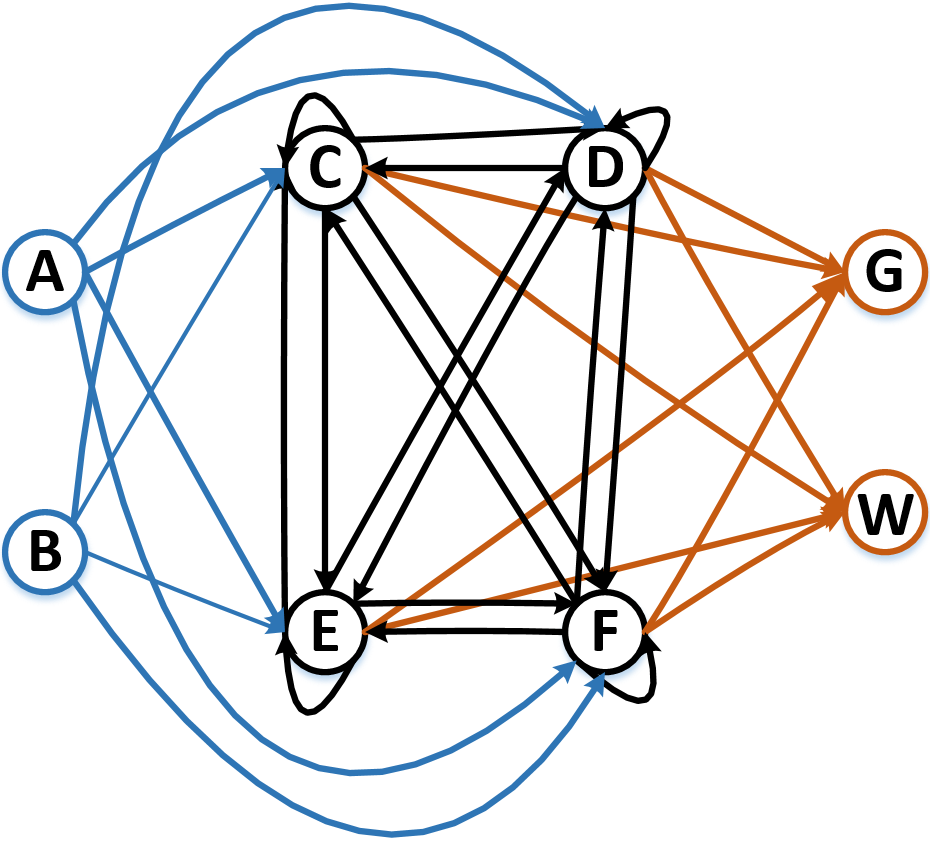
\includegraphics[scale=0.23]{figures/Fig1.png}}
	}}
      
      \caption{A Boolean control network with two input-nodes $A$ and $B$, four state-nodes $C$, $D$, $E$ and $F$, and two output-nodes $G$, $W$. We use blue, black and orange, to distinguish three types of nodes and three types of edges.}
      \label{fig:1}
  \end{figure}

%To better illustrate the concept of {\em BCNs}, we give a simple example to describe it.

\begin{example}
In Fig.\ref{fig:1} we have a \BCN\ with two input-nodes $A$ and $B$, four state-nodes $C$, $D$, $E$ and $F$, two output-nodes $G$, $W$ and the directed edges which connect them. And we have the updating rules of this \BCN\ that \[C(t), D(t), E(t), F(t)\in s(t)\] denote the value of state-nodes at time step $t$;
\[A(t), B(t)\in i(t)\] denote the value of input-nodes at time step $t$;
\[G(t), W(t)\in o(t)\] denote the value of output-nodes at time step $t$;
$f:\mathbb{B}^{6}\mapsto \mathbb{B}^4$ and $h:\mathbb{B}^4\mapsto \mathbb{B}^2$ are shown in the truth table (Fig.\ref{fig:2}).  For instance, the updating rule of output-node $G$ is 
\[G(t)=C(t)\wedge \neg(\neg{D(t)}\wedge \neg E(t)\wedge \neg F(t))\]
	
The reason why we use the truth table to describe the updating rules of the \BCN\ is that it would be will be more convenient for a \BCN\ to be converted into its aglebraic form. What's more, for convenience, we will use this example to explain various concepts throughout this paper.
  \begin{figure}[thpb]
      \centering
      \framebox{\parbox{3in}{
		\centerline{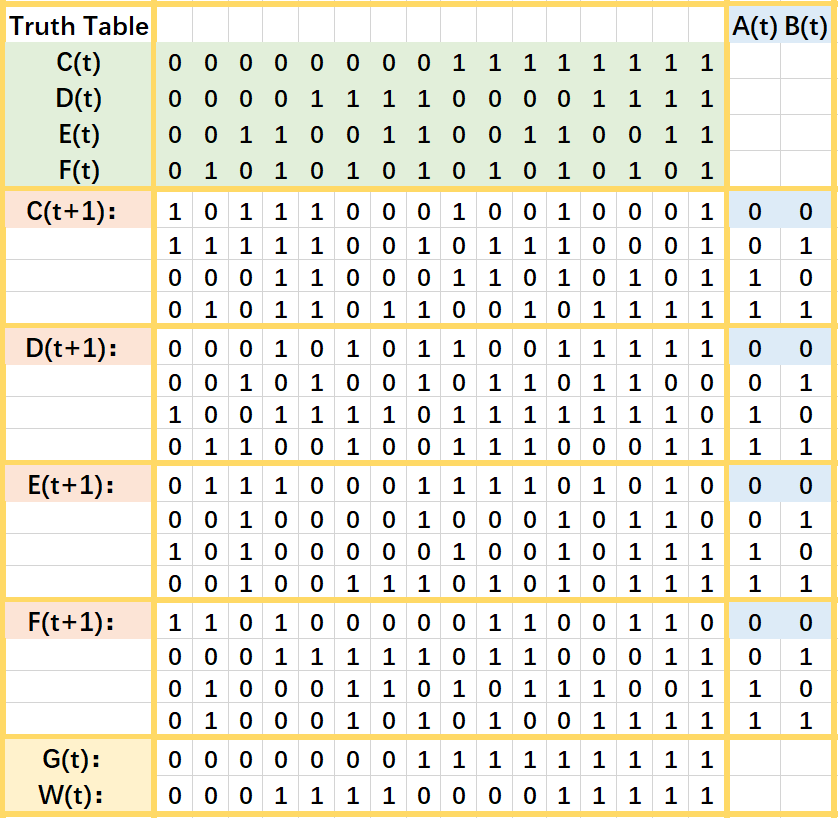
\includegraphics[scale=0.26]{figures/Fig2.png}}
	}}
      
      \caption{The truth table which describe the updating rules of the \BCN\ shown in Fig.\ref{fig:1}.}
      \label{fig:2}
   \end{figure}
   \label{exa:2}
\end{example}   


%==============================================================================================================
\subsection{The algebraic forms of \BCNs}
As mentioned in the {\em Section \ref{sec:intro}}, \STP\ is one of useful tools to deal with  both \BNs\ and \BCNs\  related problems \cite{cheng2009controllability}. The \STP\ is used to represent the algebraic form of \BCN. The algebraic form of \BCN\ helps us to introduce four existing observability of \BCN\ and define the online observability of \BCN. The definition of \STP\ is as follows.

\begin{definition}[STP] 
	\cite{Cheng2011Analysis} Let $X\in\mathbb{R}_{m\times n}$, $Y\in\mathbb{R}_{p\times q}$ and $\alpha=lcm(n,p)$ be the least common multiple of $n$ and $p$. The \STP\ of $X$ and $Y$ is defined as \[X\ltimes Y=(X\otimes I_{\alpha/n})(Y\otimes I_{\alpha/p}),\] where $\otimes$ denotes the {\em Kronecker product}. 
\end{definition}

After introducing the definition of \STP\ of matrices,  we introduce some related notations at first \cite{Zhang2016Observability}:
\begin{itemize}
  \item $\delta^i_n$: the $i$-th column of the identity matrix $I_n$;
  \item $\Delta_n$: the set $\{\delta^1_n,\ldots,\delta^n_n \}$; 
  \item $\delta_n \left[i_1,\ldots,i_s\right]$: $\left[\delta^{i_1}_n,\ldots,\delta^{i_s}_n\right]\left(i_1,\ldots,i_s\in\left\{1,2,\ldots,n\right\}\right)$ the logical matrix;
  \item  $L_{n\times s}$: the set of $n\times s$ logical matrices.
\end{itemize}

Using \STP\ of matrices, the updating rules of the \BCN\ (\ref{equ:1}) can be quivalently represented in the following algebraic form:
\begin{definition}

\begin{equation}
\begin{split}
s(t+1)=&\ L\ltimes{i(t)}\ltimes{s(t)}\\
o(t)=&\ H\ltimes{s(t)}
\end{split}
\label{equ:2}
\end{equation}
where $s(t)\in\Delta_N$, $i(t)\in\Delta_M$, and  $o(t)\in\Delta_Q$ denote the states, inputs and outputs respectively the same as in formula (\ref{equ:1}), but $s(t)$, $i(t)$ and $o(t)$ in formula (\ref{equ:2}) would be written in special vector forms; $L\in L_{N\times\left(NM\right)}$ and $H\in L_{Q\times N}$ denote the relation matrices, where $N=2^n$, $M=2^m$, and $Q=2^q$. 
\end{definition}

Since \STP\ keeps most properties of the conventional product \cite{Cheng2011Analysis}, the associative law, the distributive law, etc., we usually omit the symbol ``$\ltimes$'' hereinafter. For instance, the 
formula \[s(t+1)=L\ltimes{i(t)}\ltimes{s(t)}\] will be written as  \[s(t+1)=L{i(t)}{s(t)}.\]

After the introduction of the algebraic forms of \BCNs, we introduce the process of constructing a \BCN\' s algebraic form. In order to construct the algebraic form of \BCN\ (\ref{equ:2}) we give a mapping \[\tau:\{0,1\}\mapsto \{\delta_2^1, \delta_2^2\},\] where $\tau(0)=\delta_2^2$, $\tau(1)= \delta_2^1$. 
%each logical value a vector form as: $1 \scriptsize{\sim} \delta_2^1$, $0 \scriptsize{\sim} \delta_2^2$. 
Therefore, the logical variable $A(t)$ takes value from these two vectors, i.e., $A(t)\in \{\delta_2^1, \delta_2^2\}$. Using the \STP\ of matrices, we have 
\[i(t)=i_1(t){\ldots}i_m(t);\] 
\[s(t)=s_1(t){\ldots}s_n(t);\] 
\[o(t)=o_1(t){\ldots}o_q(t).\] 
And according to \cite{Cheng2003Semi}, for the logical function of each state-node $f_p$ which can be found in the updating rules (\ref{equ:1}). The form of  $f_p$ as:
\[f_p(i_1(t),\ldots,i_m(t),s_1(t),\ldots,s_n(t))\] 
there exists a structure matrix $L_p\in L_{2\times {NM}}$ such that
\begin{equation}
\begin{split}
\tau(f_p(i_1(t),\ldots,i_m(t),s_1(t),\ldots,s_n(t)))= L_pi(t)s(t)
\end{split}
\end{equation}
%where the left side of equation calculate the truth value and the  right side of equation calculate the vector in $\{\delta_2^1, \delta_2^2\}$. 
Therefore for state-nodes $s_1,\ldots,s_n$, we have $n$ logical matrices $L_1,\ldots,L_n$ for them, respectively. 
%We have that
%when\\
If for each state-node $s_p$ the logical matrix has its form
\[L_p=[\delta_2^{p_1},\ldots,\delta_2^{p_{NM}}],\] 
then we have that %for the set of all state-nodes $s(t)$ the logical matrix 
\[L=[\delta_N^{R_1},\ldots,\delta_N^{R_{NM}}]\]  where 
\[\delta_N^{R_1}=\delta_2^{1_1}\ldots\delta_2^{n_1};\ldots; \delta_N^{R_{NM}}=\delta_2^{1_{NM}}\ldots\delta_2^{n_{NM}}.\] 
%then 
By this relationship we can construct the $L$ for the algebraic forms of \BCNs. What's more we can also construct the logical matrix $H$ in the similar way. To better illustrate the concept of algebraic forms, we give a simple example to describe it.
\begin{example}
For instance, for the \BCN\ mentioned in {\em Example \ref{exa:2}}, we have that the updating rules of this \BCN\ can be represented with the algebraic form:
\begin{equation}
\begin{split}
s(t+1) =&\delta_{16}[\alpha]i(t)s(t)\\
o(t) =&\delta_4[\beta]s(t)\\
\end{split}
\label{equ:4}
\end{equation}
where $\alpha=\{10,4,11,16,9,5,1, 7,15,2,3,12,7,6,8,13,8,9,\\15,10,14,4,3,16,1,14,12,13,5,7,2,6,7,2,3,13,13,9,5,1,\\16,13 ,6,14,11,10,4,15,1,14 ,7,6,9 ,8,11,12,5,5,13,3,10,\\12,16,16\}$, $\beta=\{1,1,1,2,2,2,2,3,3,3,3,4,4,4,4,4\}$, $t\in \mathbb{N}$, $s\in \Delta_{16}$, $i\in \Delta_4$ and $o\in \Delta_4$.
\end{example}   
\subsection{Four existing observability of \BCNs}
After introducing the algebraic forms of \BCNs, we introduce four existing types of observability of \BCNs\ in this subsection. In order to introduce four existing types of observability of \BCNs, we define the mappings \cite{Zhang2016Observability}:
\begin{equation}
\begin{split}
L^p_{s_0} &: (\Delta_M)^p\mapsto(\Delta_N)^p, i_0\ldots i_{p-1} \mapsto s_1 \ldots\, s_p\\
L^{\infty}_{s_0} &: (\Delta_M)^{\infty}\mapsto(\Delta_N)^{\infty}, i_0 i_1 \ldots  \mapsto s_1 s_2 \ldots
\end{split}
\label{equ:5}
\end{equation}
\begin{equation}
\begin{split}
(HL)^p_{s_0} &: (\Delta_M)^p\mapsto(\Delta_Q)^p, i_0\ldots i_{p-1} \mapsto o_1\ldots\, o_p\\
(HL)^{\infty}_{s_0} &: (\Delta_M)^{\infty}\mapsto(\Delta_Q)^{\infty}, i_0 i_1 \ldots  \mapsto o_1 o_2\ldots
\end{split}
\label{equ:6}
\end{equation}

Where $\Delta_N$, $\Delta_M$ and $\Delta_Q$ are three alphabets, $s_0\in \Delta_N$, $p\in \mathbb{Z}_+$ and $\infty$ is the infinite natural numbers. For all  $p\in \mathbb{Z}_+$, \[I=i_0 \ldots i_{p-1} \in(\Delta_M)^p\] is an input sequence, \[L^p_{s_0}(I)=s_1 \ldots s_{p} \in(\Delta_N)^p\] is a state sequence and \[(HL)^p_{s_0}=o_1 \ldots o_{p} \in(\Delta_N)^p\] is a output sequence. For the $\infty$, \[I=i_0 \ldots  \in(\Delta_M)^{\infty}\] is an infinitely long input sequence, \[L^{\infty}_{s_0}(I)=s_1 \ldots  \in(\Delta_N)^{\infty}\] is an infinitely long state sequence and \[(HL)^{\infty}_{s_0}(I)=o_1 \ldots \in(\Delta_N)^{\infty}\] is an infinitely long output sequence. From the algebraic forms of \BCNs, in the formula (\ref{equ:5}), for any $1\le k \le |I|$ we have \[s_k=Li_{k-1}s_{k-1}.\] In the formula (\ref{equ:5}) and formula (\ref{equ:6}), for any $1\le k \le |I|$ we have  \[o_k=Hs_k=HLi_{k-1}s_{k-1}.\] Then four existing types of observability of BCNs can be define as follows.
%And for all $1\ge k \ge j \ge |I|$, we use I[k,j] to denote the word $i_k \ldots i_j$ as an input sequence. 
\begin{definition}
The first type of observability is that, \BCN\ is called observable, if for every initial state $s_0 \in \Delta_N$, there exists an input sequence $I\in(\Delta_M)^p$ for some $p\in \mathbb{Z}_+$ such that for every two states $s_0\neq {s'}_0\in \Delta_N$, $Hs_0=H{s'}_0$ implies $(HL)^p_{s_0}(I)\neq (HL)^p_{{s'}_0}(I)$ \cite{cheng2009controllability}.
\end{definition}

Hence the first observability means that if a \BCN\ is observable then every initial state of the \BCN\ can be determined by an input sequence. But we can only use the corresponding input sequence $I$ of a state $s_0$ to check whether it is the initial state of this \BCN\ or not.
\begin{example}
For example, for the \BCN\ mentioned in {\em Example \ref{exa:2}}, we have for every initial state of this \BCN\ can be determined by an input sequence.  For instance,
\begin{itemize}
  \item the state $\delta_{16}^1$ can be determined by any input sequence which with the prefix $\delta_{4}^4$, $\delta_{4}^1 \delta_{4}^3$ and $\delta_{4}^1 \delta_{4}^4$, etc;
  \item the state $\delta_{16}^2$ can be determined by any input sequence which with the prefix $\delta_{4}^1$, $\delta_{4}^3$ and $\delta_{4}^4$, etc;
  \item the state $\delta_{16}^2$ can be determined by any input sequence which with the prefix $\delta_{4}^2$, $\delta_{4}^4$and $\delta_{4}^1 \delta_{4}^4$, etc.
\end{itemize} 
Therefore we have this \BCN\ satisfies the existing first observability.
\end{example}   

\begin{definition}
	The second type of observability is that, a \BCN\ is called observable if for any distinct states $s_0$, ${s'}_0 \in \Delta_N$, there exists an input sequence $I\in(\Delta_M)^p$ for some $p\in \mathbb{Z}_+$, such that $Hs_0=H{s'}_0$ implies $(HL)^p_{s_0}(I)\neq (HL)^p_{{s'}_0}(I)$ \cite{Zhao2010Input}.
\end{definition}

The second observability means that a \BCN\ is called observable if for every two distinct initial states $s_0, s_0'$of the \BCN, there exists an input sequence $I$ which can distinguish them. 
\begin{example}
For example, for the \BCN\ mentioned in {\em Example \ref{exa:2}}, we have for every two distinct initial states of the \BCN, there exists an input sequence which can distinguish them.  For instance,
\begin{itemize}
  \item the states $\delta_{16}^1$ and $\delta_{16}^2$ can be distinguished by any input sequence which with the prefix $\delta_{4}^1$, $\delta_{4}^2 \delta_{4}^1$ and $\delta_{4}^2 \delta_{4}^2$, etc;
  \item the states $\delta_{16}^1$ and $\delta_{16}^3$  can be distinguished by any input sequence which with the prefix $\delta_{4}^2$, $\delta_{4}^3$ and $\delta_{4}^4$, etc;
  \item the states $\delta_{16}^2$ and $\delta_{16}^3$  can be distinguished by any input sequence which with the prefix $\delta_{4}^1$, $\delta_{4}^2$and $\delta_{4}^4$, etc.
\end{itemize} 
Therefore we have this \BCN\ satisfies the existing second observability.
\end{example}   
\begin{definition}
The third type of observability is that, a \BCN\ is called observable if there exists an input sequence $I\in(\Delta_M)^p$ for some $p\in \mathbb{Z}_+$, such that for any distinct states $s_0$, ${s'}_0 \in \Delta_N$, $Hs_0=H{s'}_0$ implies $(HL)^p_{s_0}(I)\neq (HL)^p_{{s'}_0}(I)$ \cite{Cheng2011Identification}.
\end{definition}

The third observability means that a \BCN\ is called observable if there exists an infinitely long input sequence which can determine the initial state $s_0$ of the \BCN\ for every $s_0\in\Delta_N$.

\begin{example}
For example, for the \BCN\ mentioned in {\em Example \ref{exa:2}}, we have there is an input sequence which can determine the initial state of this \BCN.  For instance, any input sequence which with the prefix $\delta_{4}^1\delta_{4}^4\delta_{4}^1$ can determine the initial state of this \BCN.

Therefore we have this \BCN\ satisfies the existing third observability.
\end{example}  
\begin{definition}
	The fourth type of observability is that, \BCN\ is called observable, if for any distinct states $s_0$, ${s'}_0 \in \Delta_N$, for any input sequence $I\in(\Delta_M)^{\infty}$, $Hs_0=H{s'}_0$ implies $(HL)^{\infty}_{s_0}(I)\neq (HL)^{\infty}_{{s'}_0}(I)$ \cite{Fornasini2013Observability}.
\end{definition}

The fourth observability means that a \BCN\ is called observable if every sufficient long input sequence can determine the initial state $s_0$ of the \BCN\ for every $s_0\in\Delta_N$.
\begin{example}
In the previously mentioned \BCN. There exists at least one sufficient long input sequence can not determine the initial state of this \BCN. For instance, the states $\delta_{16}^4$ and $\delta_{16}^5$  will convert into $\delta_{16}^{13}$ after being affected by $\delta_{4}^3$, therefore any input sequence which with the prefix $\delta_{4}^3$, they can not determine the initial state $s_0$ of the \BCN\ for every $s_0\in\Delta_N$.

Therefore we have this \BCN\ satisfies the existing fourth observability.
\end{example}  

What is more, we know the implication relationships of four existing types of observability from the definitions of them \cite{Zhang2016Observability}. 
\begin{proposition}
The implication relationships of four existing types of observability.
\begin{itemize}
\item The first observability implies the second observability, but the second observability does not imply the first observability.\\
\item The third observability implies the second observability, but the second observability does not imply the third observability.\\
\item The third observability implies the first observability, but the first observability does not imply the third observability.\\
\item The fourth observability implies the third observability, but the third observability does not imply the fourth observability.\\
\item The fourth observability implies the second observability, but the second observability does not imply the fourth observability.\\
\item The fourth observability implies the first observability, but the first observability does not imply the fourth observability. \\
\end{itemize} 
\end{proposition}

Where the implication relationship is that ``The first observability implies the second observability.'' means ``If a \BCN\ satisfies the first observability then it satisfies the second observability.'' For the details of the proving process of this proposition, we refer readers to \cite{Zhang2016Observability}.
%, when we don't presuppose the initial state of {\em BCNs}
 
When we want to determine the initial state of some \BCNs\ by four existing types of observability. The first and second observability can not help us to determine the initial state of some \BCNs\ which can be checked at most once. For example, in the first type observability we need to assume that the initial state $s_0$ of a \BCN\ is $s_i$, and then check it by corresponding input sequence $I_i$ of this state. If the initial state we assume is correct, then we can determine the initial state $s_0=s_i$. But if the assumption is not correct, we can not determine the initial state of the \BCN. Therefore we need to check several test cases (with the same initial state $s_0$) of this \BCN\ untill we can determine the initial state of them. However we can use the third existing observability and fourth existing observability to determine the initial state of \BCNs\ through one test case. That we need not to presuppose the initial state of \BCNs\ when we use the third observability and fourth observability. But the requirements for \BCNs\ are very harsh when we use the third observability and fourth observability.
 
In some biological systems, the initial state of them can be checked at most once, i.e., we can only check the initial state of some biological systems (depicted by \BCNs) in real time. Therefore, we can not use the first observability and second observability to determine the initial states of them in real time. Moreover, in some biological systems, it would takes many costs to check these biological systems. Hence we will spend a lot of overhead to determine the initial states of them by the first observability and second observability. Furthermore, we also can not use the third observability and fourth observability to determine the initial states of some biological systems if they can not satify the requirements of the third and fourth observability. With these disadvantages of four existing observability, we propose the online observability of \BCNs\ to solve this problem.
 \subsubsection*{Problem}
Finding the necessary and sufficient condition of determine the initial state $s_0$ of \BCNs\ in real time for every $s_0\in \Delta_N$.